% !TEX root = template.tex

\section{Results}
\label{sec:results}

The results we show span the various architectures and methods we tried during the course of the project.

\subsection{Baseline Model with BCE loss}
In this first experiment we trained the baseline model with BCE loss. 
In Fig.~\ref{fig:accuracy_bce} we show the curves of the accuracy of the Discriminator. We can see that after just a few epochs this curve directly went to 1, meaning that the Generator was never able to produce valid bars of music.

\begin{figure}[!h]
    \centering
    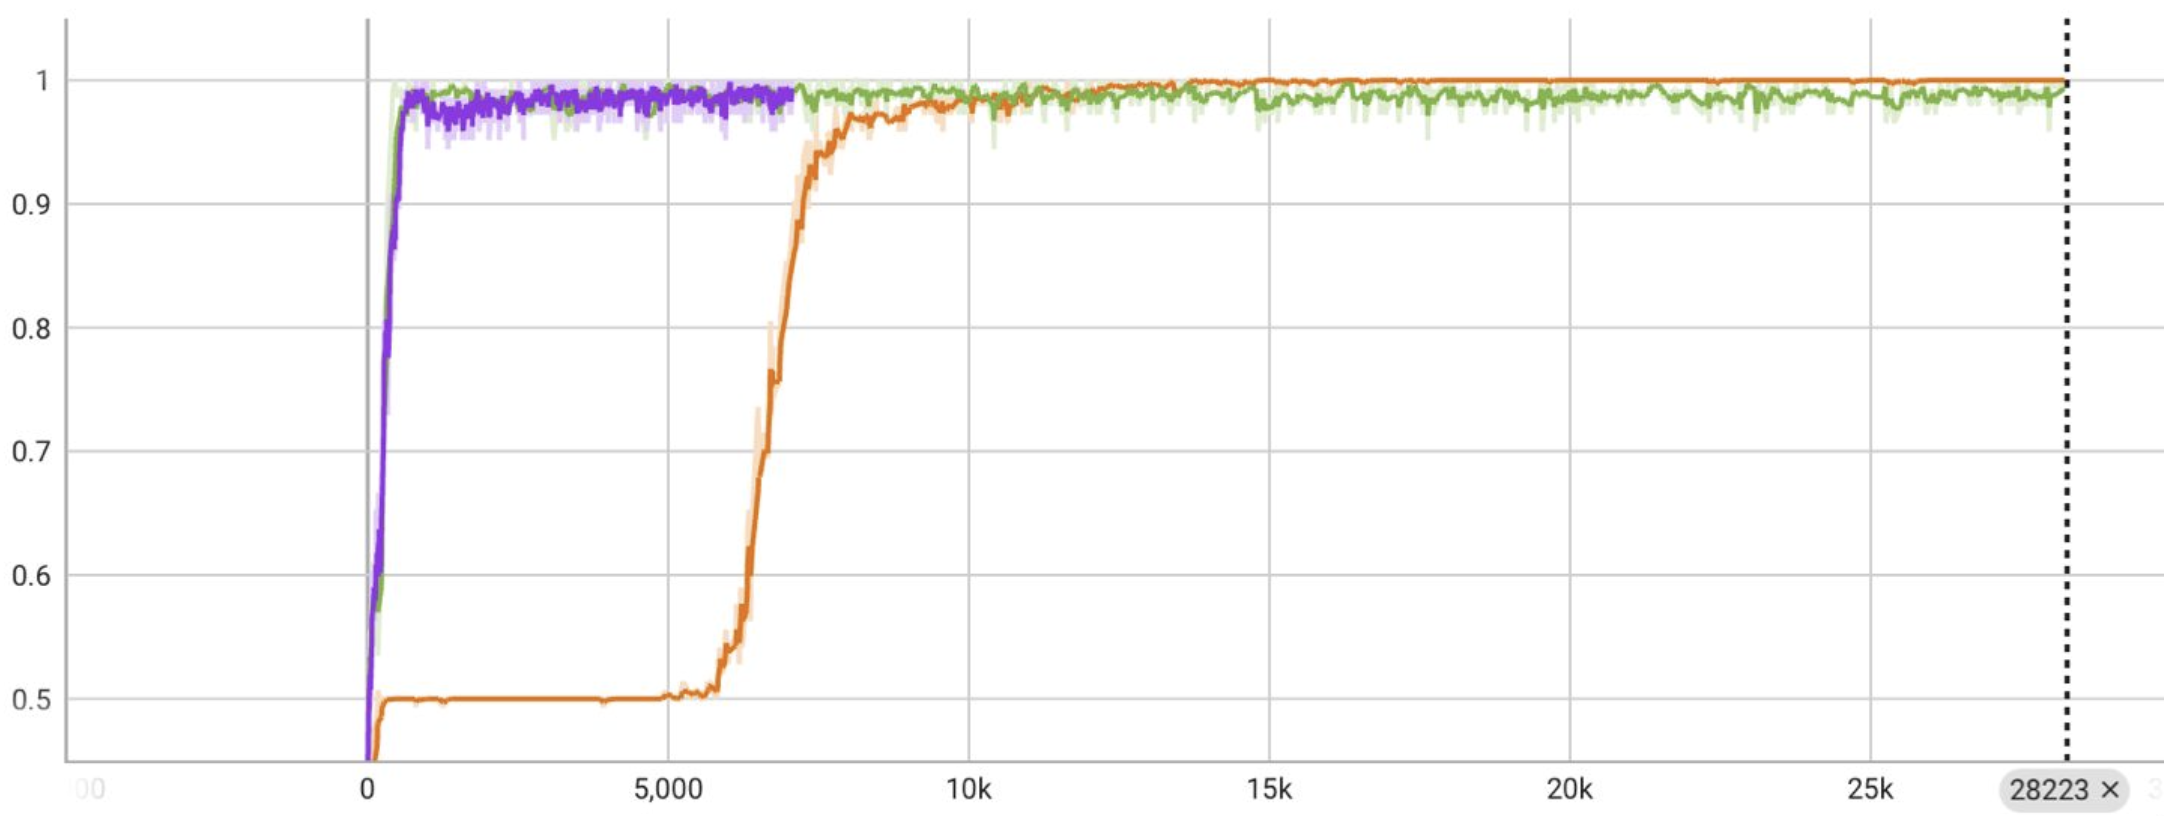
\includegraphics[width=\linewidth]{images/accuracy_BCE.png}
    \caption{Discriminator accuracy during the baseline training with BCE loss. The rapid convergence to 1 indicates that the Generator was immediately outperformed, leading to vanishing gradients.}
    \label{fig:accuracy_bce}
\end{figure}

The most delayed curve is the one corresponding to the introduction of the residual layers. Here the accuracy was able to stay around 0.5 for a few epochs, but then eventually collapsed to 1. At this point, the music produced was completely random.

\subsection{Improved Model with WGAN-GP loss}
The next step was the introduction of the WGAN-GP loss. Now, additionally to the generator and critic losses, we also tracked the \textit{Wasserstein distance estimation} and the \textit{feature matching loss}.

The idea of the first metric is that it should slowly decrease and stabilise towards zero, indicating indistinguishable distributions. Too high values indicate a too strong Critic, while too low negative values may indicate mode collapse, as the Critic is assigning too high values to the generated music

Regarding the feature matching loss, this also should slowly decrease towards low values, as it shows that the Generator is able to reproduce correctly the statistics of the real distribution. We first started with a weight of $5.0$, but gradually decrised to $0.1$ as we noticed that high values were favoring the model in reproducing average dataset statistics over diverse music, always leading to similar patterns (mode collapse).
This means that in. the last trainings this metric was less used.

At this point, even if the game seemed more balanced, the Generator was always able to produce music that fooled the Discriminator, leading to an early mode collapse.
It can be intersting to see how the loss of the generator always seemed to stay close to 0, with the critic loss being the one that fluctuated more. Looking at the produced music, we noticed that this was probably an indication of the Generator producing the same pattern over and over again, a clear signal of mode collapse.
In Fig.~\ref{fig:g_loss_collapse} and Fig.~\ref{fig:d_loss_collapse} are shown the behaviour of the two losses during training.

\begin{figure}[!h]
    \centering
    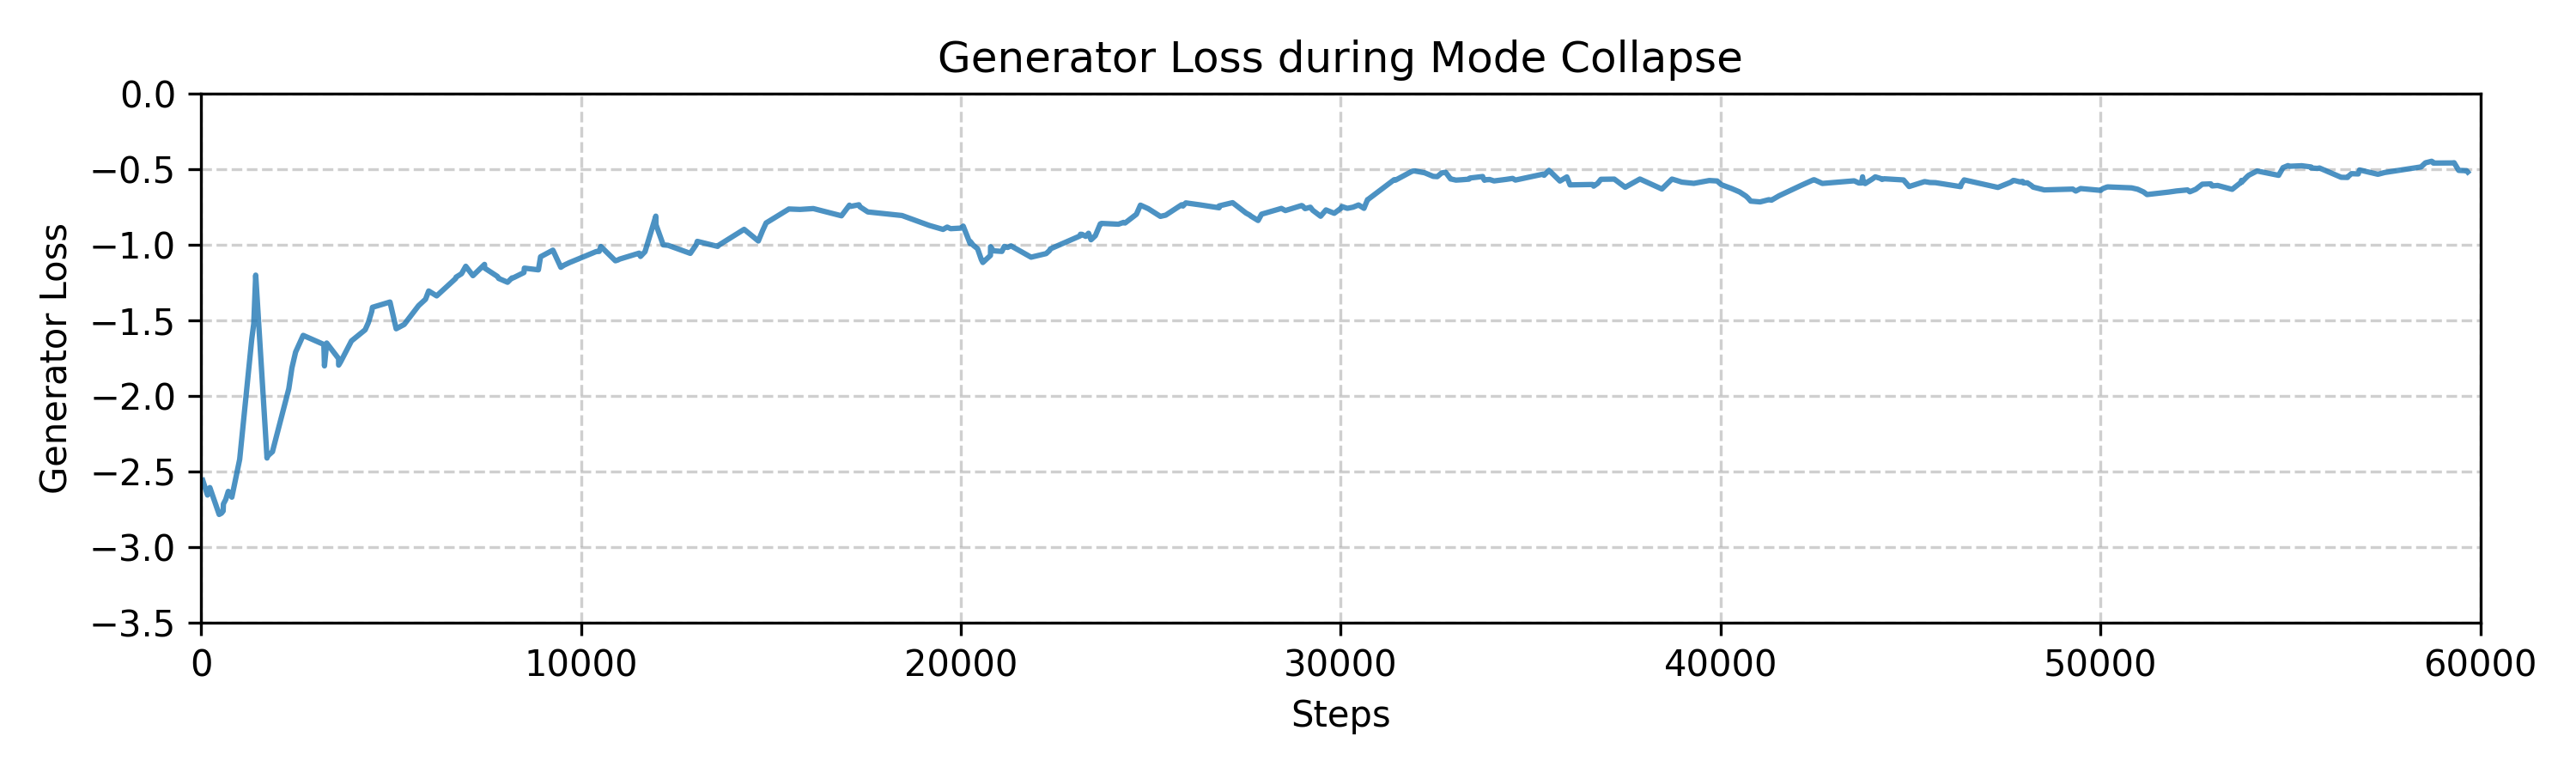
\includegraphics[width=0.9\linewidth]{images/g_loss_collapse.png}
    \caption{Generator loss curve. It remains relatively stable and close to zero.}
    \label{fig:g_loss_collapse}
\end{figure}

\begin{figure}[!h]
    \centering
    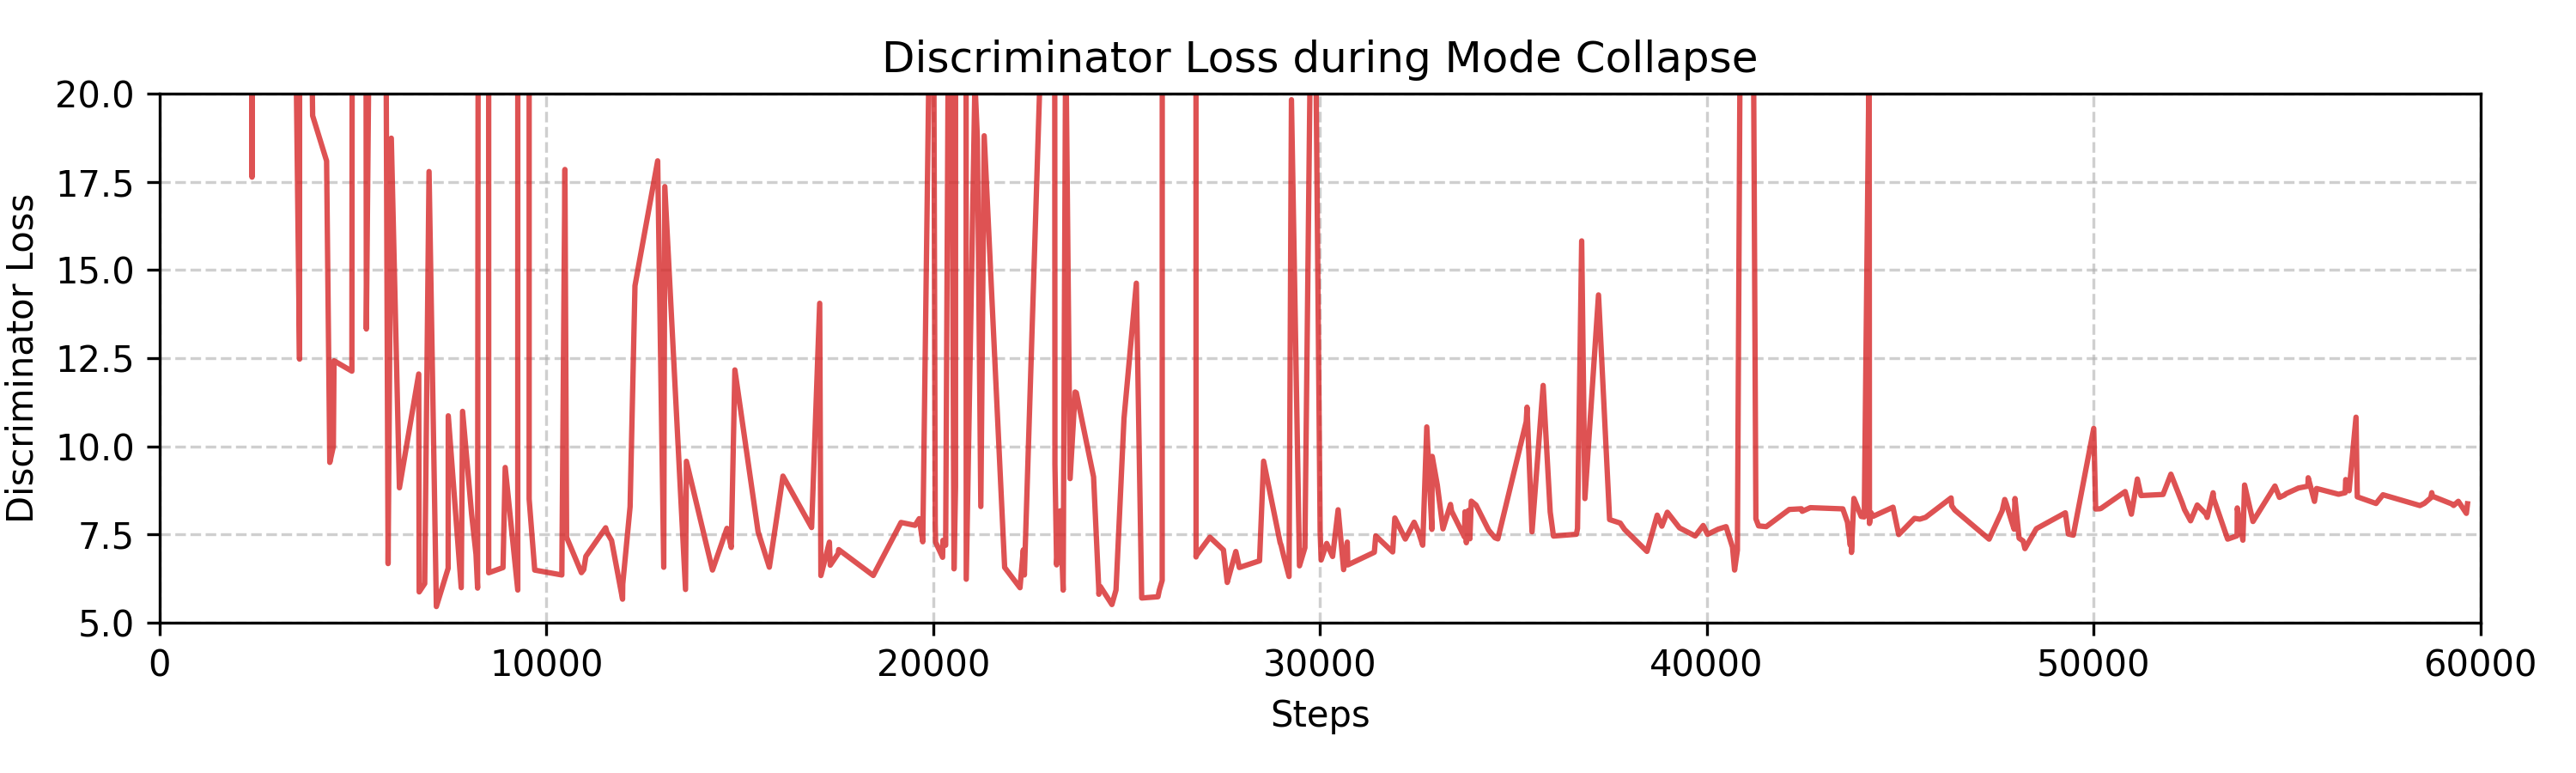
\includegraphics[width=0.9\linewidth]{images/d_loss_collapse.png}
    \caption{Discriminator loss curve. The zoom on the [0, 20] range allows to observe the spikes and fluctuations with respect to the Generator loss.}
    \label{fig:d_loss_collapse}
\end{figure}

Additionally, we also tried to produce some music at this point, as shown in Fig.~\ref{fig:piano_roll_collapse}.  The main pattern is clearly a single set of close notes continuously repeated.
\begin{figure}[!h]
    \centering
    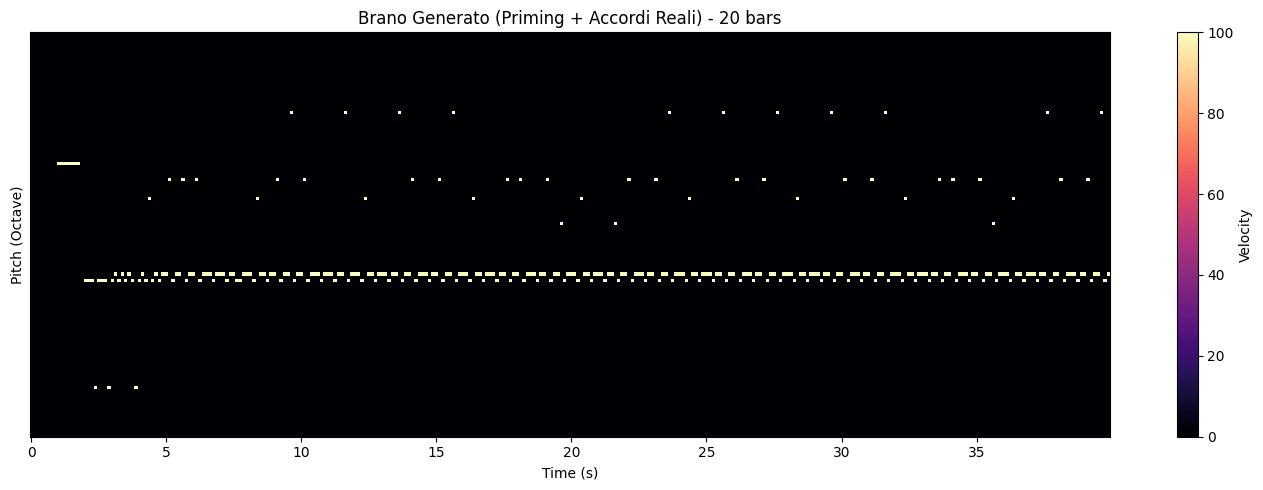
\includegraphics[width=0.9\linewidth]{images/piano_roll_collapse.jpeg}
    \caption{Generated piano roll on one of the test music.}
    \label{fig:piano_roll_collapse}
\end{figure}

\subsection{Improved Critic with minibatch std}

At this point we tried to refine the Critic's architecture as the collapsing problem was probably caused by its inability in extracting meaningful features from the produced music. We modified it into a deeper network, adding the stages we explained in \ref{sec:model_architecture}, with the objective of allowing it to extract more complex features from the music.
Additionally, to force the Generator to produce more diverse music, we tried adding the minibatch standard deviation layer. This combination led to a more active learning curve regarding the Generator and Discriminator losses and an overall more stable behaviour of the Wasserstein distance.
Here we also introduced the possibility for the Critic to perform a predefined number of updates for each update of the Generator, which allowed us to control more the balance between the two networks. In this final training it was se to $5$.
\begin{figure}[!h]
    \centering
    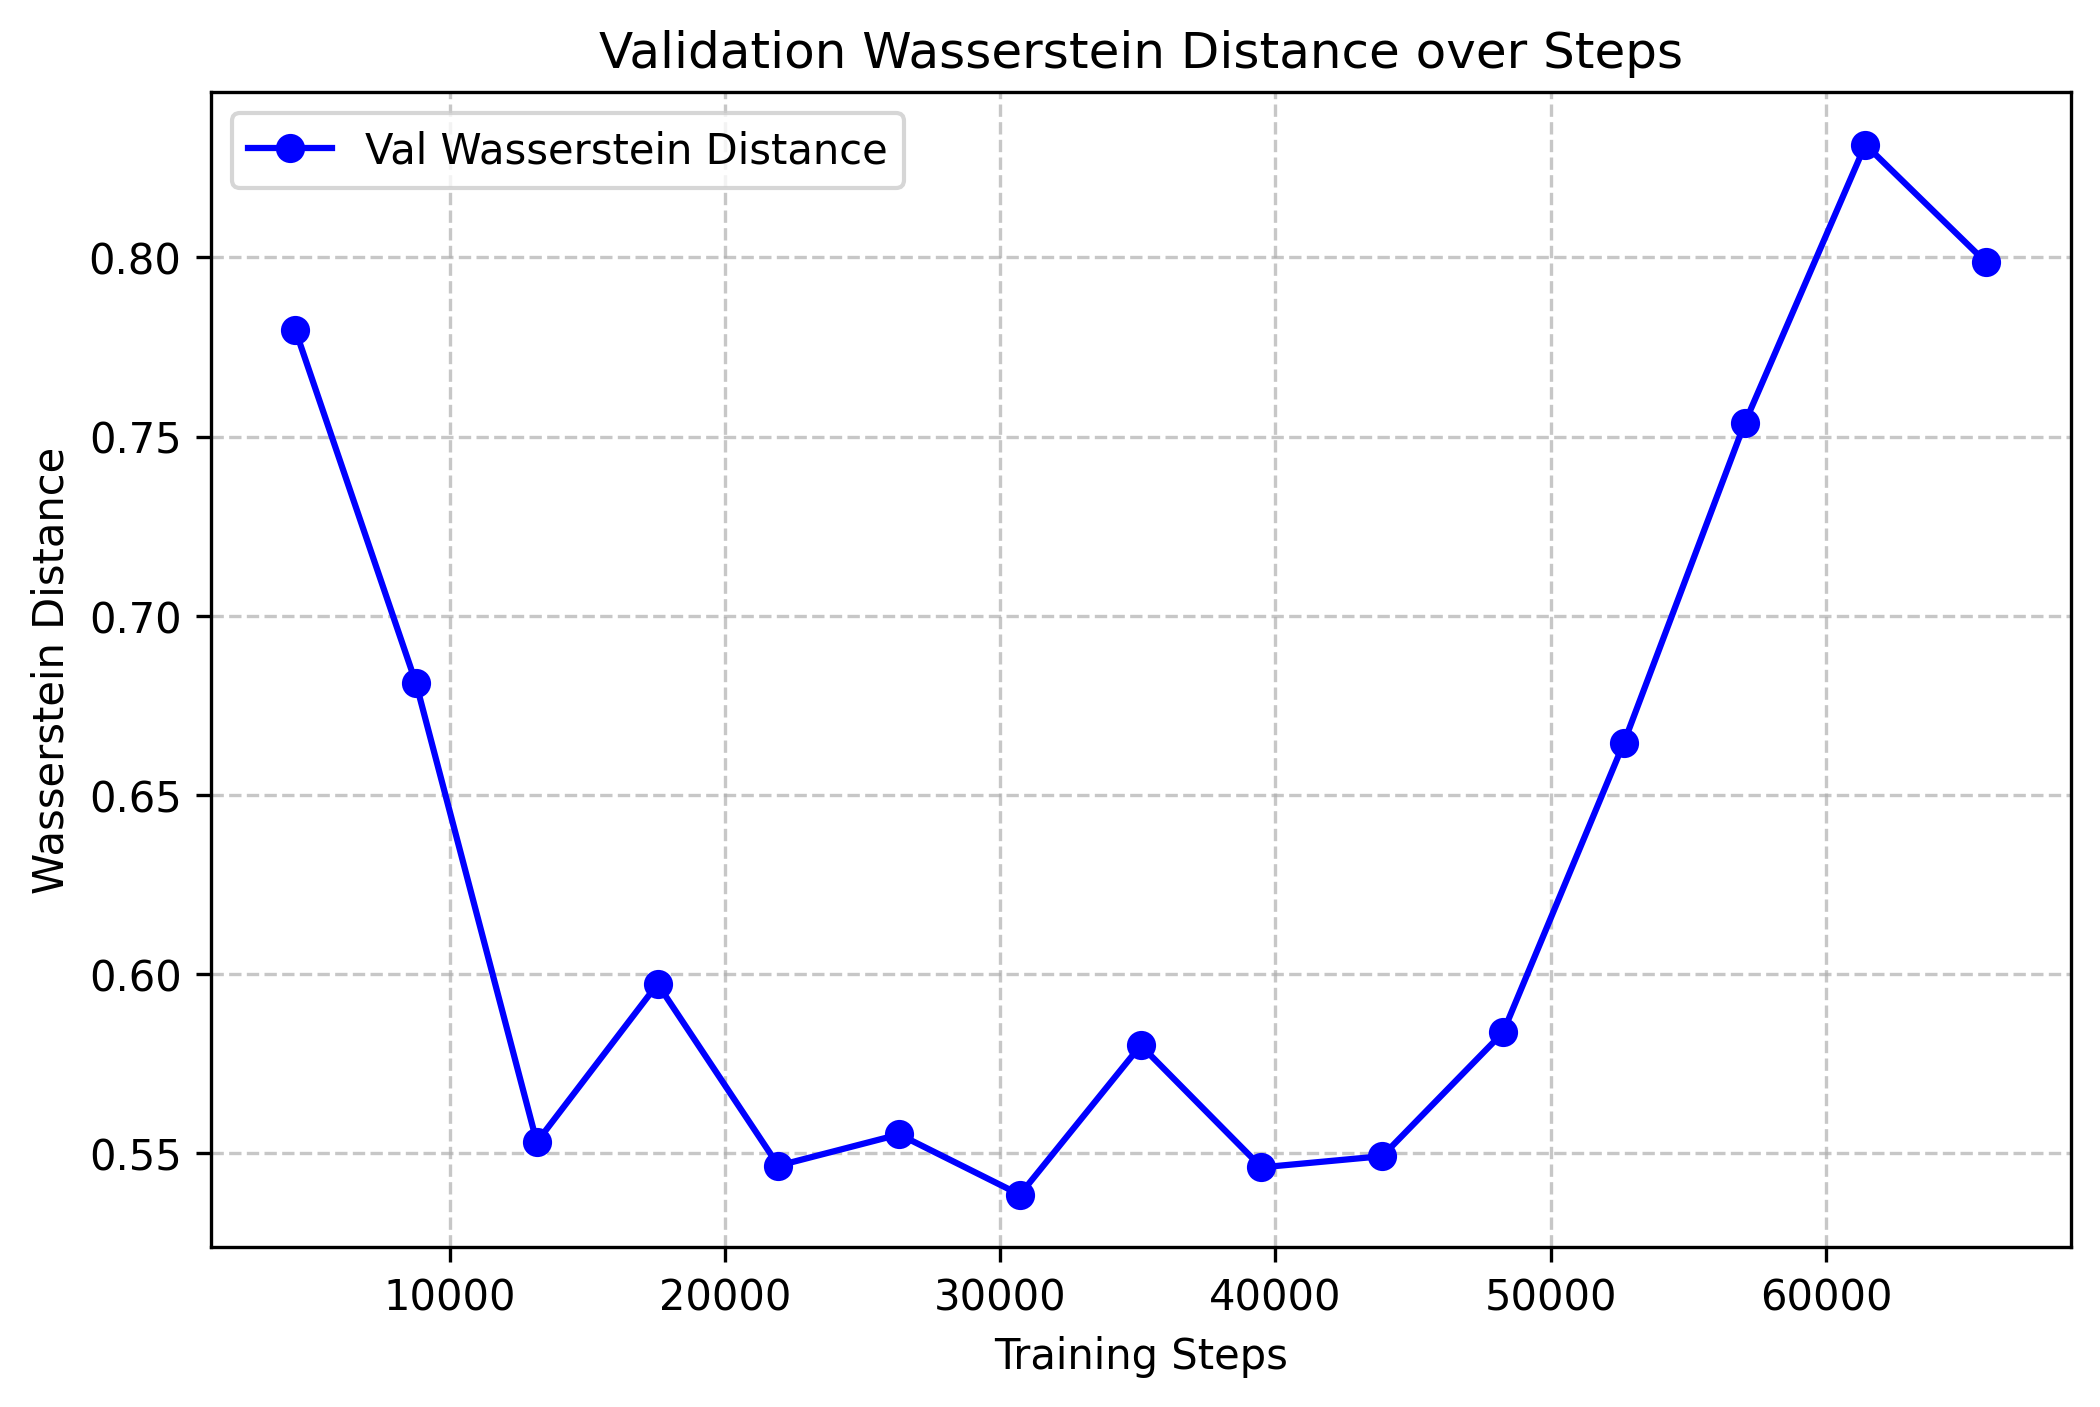
\includegraphics[width=0.7\linewidth]{images/val_w_distance.png}
    \caption{Validation Wasserstein distance during training. The initial decrease shows the model learning the distribution, while the subsequent increase suggests a potential imbalance between the Generator and the Critic.}
    \label{fig:val_w_distance}
\end{figure}

Shown in Fig.~\ref{fig:val_w_distance}, is actually the behaviour of this metric on the validation set. It reveals an interesting training dynamic. 
This training is done for 15 epochs, with the feature matching weight set to $0$, as we noticed it was not providing anymore useful results.
Initially, the distance decreases, indicating that the Generator is successfully learning to approximate the real data distribution. 
However, after approximately 40,000 steps, this curve tends to increase, suggesting that the Critic is becoming significantly more effective than the Generator.
This result shows that the model is capable of learning the real dynamics, but probably some fine tuning on the hyperparameters is still needed to reach a stable qeuilibrium and allow for longer trainings.
The results that we show in the following figures are obtained with the model at a low point on the validation curve of the validation Wasserstein distance.

\begin{figure*}[!t]
    \centering
    \begin{subfigure}{0.48\textwidth}
        \centering
        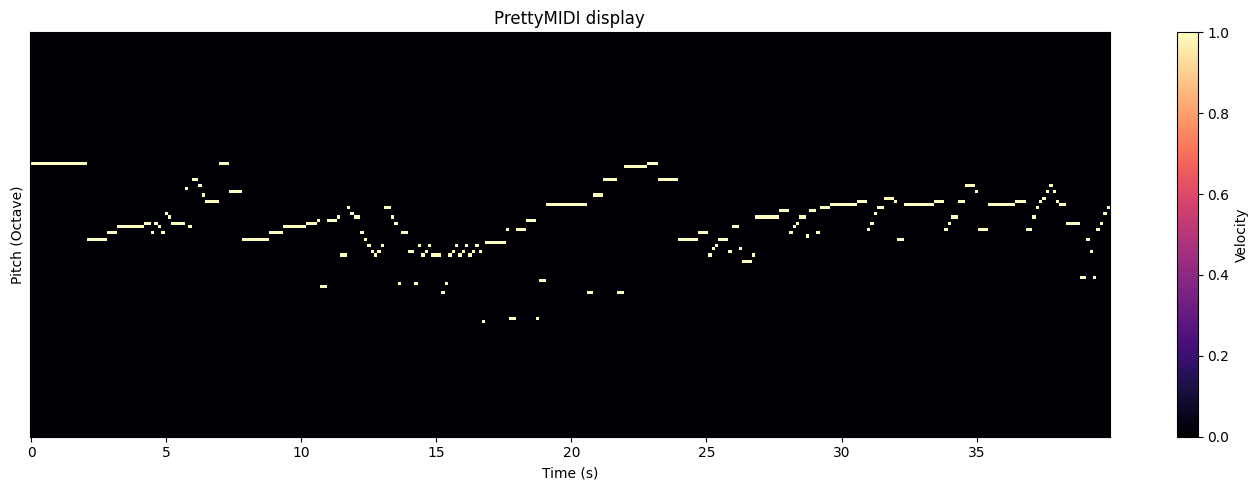
\includegraphics[width=\linewidth]{images/output_true.png}
        \caption{Ground truth sample 1 from the MAESTRO dataset.}
        \label{fig:output_true_1}
    \end{subfigure}
    \hfill
    \begin{subfigure}{0.48\textwidth}
        \centering
        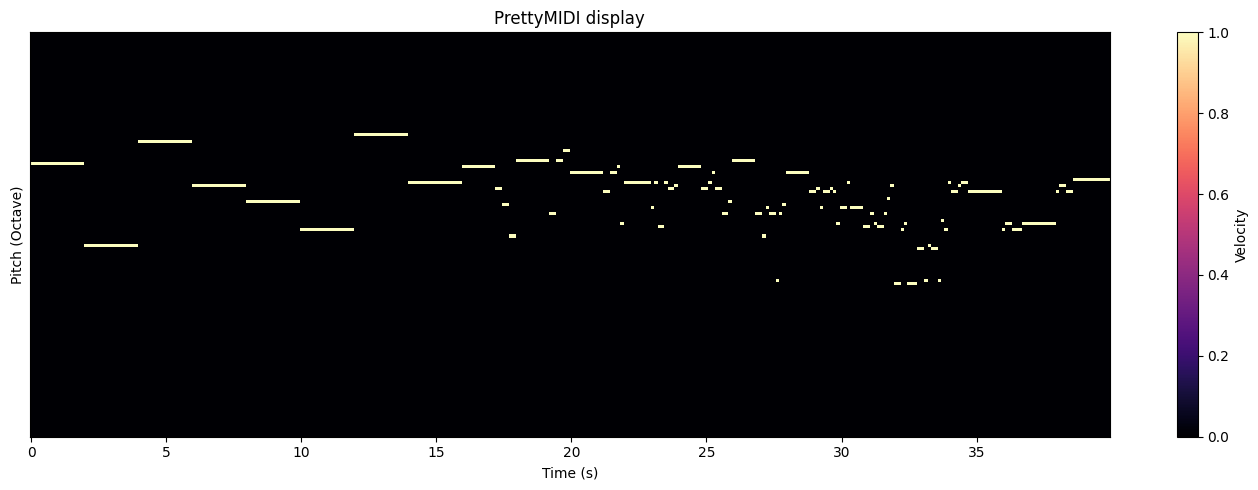
\includegraphics[width=\linewidth]{images/output_generated.png}
        \caption{Sample 1 generated by our final PianoGAN model.}
        \label{fig:output_generated_1}
    \end{subfigure}
    
    \vspace{0.4cm}
    
    \begin{subfigure}{0.48\textwidth}
        \centering
        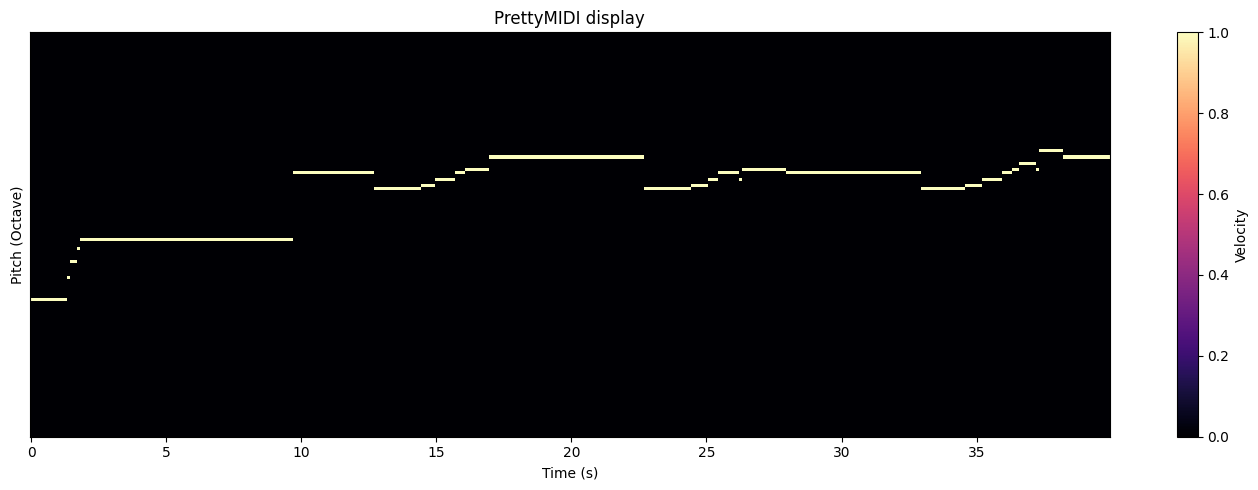
\includegraphics[width=\linewidth]{images/output_true_2.png}
        \caption{Ground truth sample 2 from the MAESTRO dataset.}
        \label{fig:output_true_2}
    \end{subfigure}
    \hfill
    \begin{subfigure}{0.48\textwidth}
        \centering
        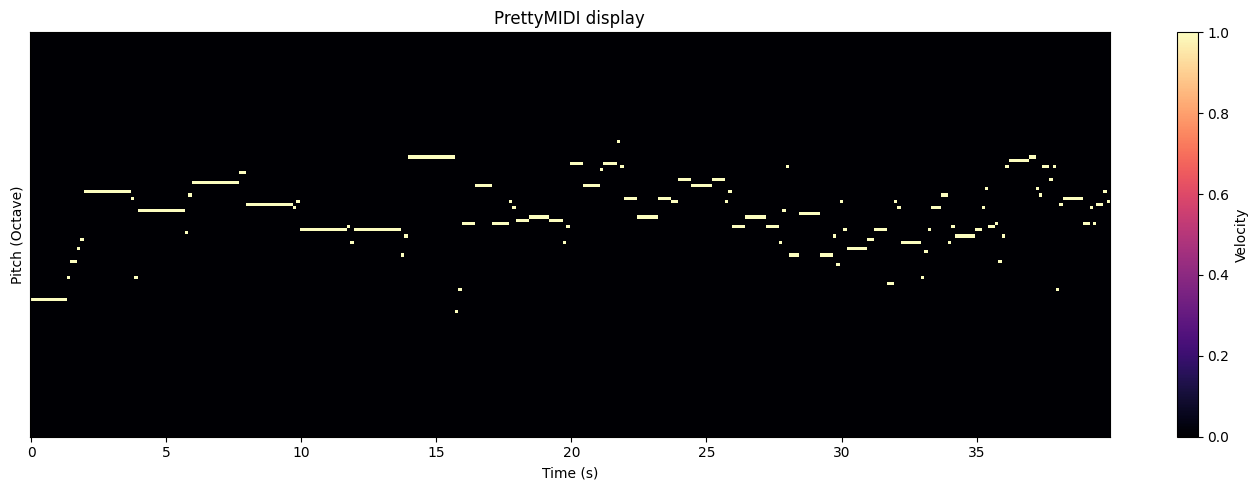
\includegraphics[width=\linewidth]{images/output_generated_2.png}
        \caption{Sample 2 generated by our final PianoGAN model.}
        \label{fig:output_generated_2}
    \end{subfigure}
    \caption{Visual comparison between real and generated piano rolls. The model successfully captures the rhythmic density and the chordal structure defined by the input conditioning.}
    \label{fig:output_comparison}
\end{figure*}


To obtain this result, we used one of the test samples from MAESTRO dataset and progressively produced 20 bars of music, each conditioned on the previously generated bar and on the underlying chord provided by the specific piece of music.
The result is a music that seems to really be conditioned on the underlying chord progression and previous bars, with no mode collapse or random note generation, as can be seen in Fig.~\ref{fig:output_comparison}.
